\section{Units}

There are four different unit types in the game: mobs, towers, projectiles and snowballs. All of these classes extend the abstract class Unit. This class contains the methods and variables that the units have in common. A Unit object contains three instance variables that are set upon creation; height, width and coordinate.

Coordinate is a helper class created to represent and manipulate the coordinates of a unit. An instance of the Coordinate class has two instance variables; x-position and y-position. To make handling of coordinates easier, there is a static method called getAngle() that calculates the angle between two coordinates that are given as parameters.

The method getDistance() returns the distance between two coordinates. The algorithm is an implementation of the Pythagorean theorem (figure ~\ref{fig:codeExGetDistance}).

%----
%- Code snippet getDistance
%----
\begin{figure}[htb]
\begin{small}
\verbatiminput{code/getDistance.java}
\end{small}
\caption{Caption}
\label{fig:codeExGetDistance}
\end{figure}
%----

\subsection{Towers}

Tower is an abstract class, that is extended by the four different tower type classes. The Tower constructor takes a coordinate as argument. The rest of the properties of a tower are specific for each tower type and therefore not set by the Tower superclass. 

Some of the methods of the Tower class are abstract. These methods are implemented in the different subclasses. These methods are setImageByLevel(), getUpgradeCost(), shoot(), createProjectile() and upgrade(). 

Since towers are stationary units, they have no method that updates their position. Instead, they have a method called tryToShoot() that is invoked everytime the updateModel() method in GameView is invoked. This method returns a new Projectile object if the tower is allowed to shoot. Towers are allowed to shoot if they are not on cooldown, and have a valid mob within their range. Some tower types have restrictions for what mob types they are allowed to target. When a tower creates a projectile, the tower is automatically set on cooldown for a specific time.

If the tower is allowed to shoot it calls the method shoot(). Basically, the shoot() method iterates over all mobs on the map and to find mobs within shooting range. Mobs that have walked a longer distance on the path are prioritized higher when the tower chooses its target. When a target has been chosen, the method creates and returns a projectile aimed at that target.

The tower is upgraded by invoking the method upgrade(). The upgrade() method increases the level of the tower by one. It then fetches the new attributes from an array of predefined values, using the level number as index.

\subsection{Mobs}

Each mob is represented by an object of the Mob class. The implementation of mobs differ from that of towers. Instead of using subclasses for each mob type, only one class is used. The mob type is set in the constructor, which is only invoked by MobFactory. The most important attributes of the Mob class are shown below.

\begin{itemize}

\item {\bf mMaxHealth:} The maximum health of the mob.
\item {\bf mHealth:} Current health of the mob. Never bigger then mMaxHealth.
\item {\bf mAngle:} Current angle toward the next checkpoint.
\item {\bf mSpeed:} Movement speed of the mob.
\item {\bf mRevard:} Money rewarded for killing the mob. Derived from the maximum health.
\item {\bf mType: } Mob type (normal, air, fast, immune or healthy).
\item {\bf mDistanceWalked:} Keeps track of how far the mob has walked.
\item {\bf mobImage:} A reference to the image to be drawn on the map.
\item {\bf mPath:} The path that the mob follows across the map.
\item {\bf mCheckpoint:} The index of the current checkpoint the mob is walking toward.

\end{itemize}

Mob contains a method called updatePosition(), which moves the mob according to its speed and its current angle. If the mob has reached its current checkpoint, the method also updates the angle to make it point toward the next checkpoint of the path. The updatePosition() method is invoked from updateModel() in the class GameView. When the last checkpoint has been passed by the mob, updatePosition() will return false. This means that the mob has survived walking to the ocean. The mob will be removed from the GameModel, the player will lose one life, and a splash animation will be displayed.

\subsubsection{Mob creation using MobFactory}

The initiation of mob waves is handled by the singleton class MobFactory. A singleton is a class that only has one instance. \citep{designPatterns}

MobFactory is initiated when the player chooses a track to play from the progression map. When a new object of the class GameView is instantiated, the method startTrack() is invoked. This method invokes getInstance() in MobFactory ensuring that the singleton instance of the class exists. When MobFactory has been initiated, a context must be set using the setContext() method. This is required to be able to reach the resources that contains the XML-file initwaves.

When the method setContext() is invoked, the private method initWaves() is also invoked. This method reads the file initwaves, which is structured as can be seen in figure ~\ref{fig:codeExInitWavesXML}.


%---------
%- Code snippet initiate waves
%---------
\begin{figure}[htb]

\begin{small}
\verbatiminput{code/initwavesXML.java}
\end{small}

\caption{Caption}
\label{fig:codeExInitWavesXML}

\end{figure}
%---------

The file initwaves contains information about every wave for every track. The XML-code is interpreted by initWaves() as a number of string arrays. Each array represents all waves in one track. Each element in an array holds information about one specific mob wave: the mob type, the number of mobs and the health of these mobs. The information is in the form of a string, and the three different values are separated by the space delimiter.

Starting from track one, initWaves() iterates until a break command is given. This occurs when the counter of the loop exceeds the number of tracks in the XML-file. Each track is identified with a dynamic string that is parsed using the methods getIdentifier() and getStringArray().

The method getStringArray() returns a string array where each element represents an item in the XML-file. A loop iterates over this array and splits each element into three separate strings: mob type, number of mobs and mob health. These strings are handled as shown in the code snippet in figure ~\ref{fig:codeExMobCreationWave}.

%---------
%- Code snippet mob creation
%---------
\begin{figure}[htb]

\begin{small}
\verbatiminput{code/mobCreationWave.java}
\end{small}

\caption{Caption}
\label{fig:codeExMobCreationWave}

\end{figure}
%---------

When the string has been processed, the correct number of mobs are created and stored in an ArrayList. When all mobs in the wave have been created, the list of mobs is stored in another ArrayList to distinguish it from waves that belong to different tracks. This is visualized in figure ~\ref{fig:dataStructureWave}.

%------
%- Image wave data structure
%------
\begin{figure}[here]

\begin{center}
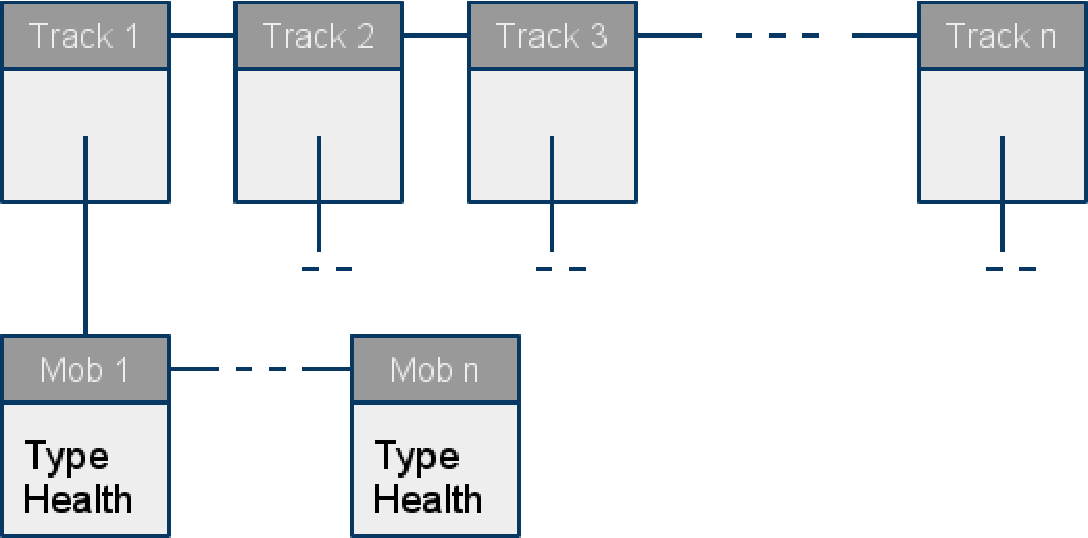
\includegraphics[scale=0.5]{pics/chapters/chapter4/moblist2}
\end{center}

\caption{Data structure of a wave object}
\label{fig:dataStructureWave}

\end{figure}
%------

MobFactory provides a method called getNextMob() that returns the next mob that should enter the game field. Since getNextMob() is invoked continuously, a delay is implemented (figure ~\ref{fig:codeExWaveDelay}) to make sure the mobs do not flood the game field completely. This is done by counting the number of times the method is invoked, only returning a new mob when the method has been invoked a certain number of times.

%---------
%- Code snippet wavedelay
%---------
\begin{figure}[htb]

\begin{small}
\verbatiminput{code/waveDelay.java}
\end{small}

\caption{Caption}
\label{fig:codeExWaveDelay}

\end{figure}
%---------

\subsection{Projectiles}

There are four types of projectiles, one for each tower type. They all extend the abstract class Projectile. When a tower shoots at a mob it creates a projectile that moves toward the mob and inflicts damage to it. The projectile has a specific mob as target and is angled toward the position of that mob. For all projectile types except the SplashProjectile this angle is updated every time updatePosition() is invoked to make sure it will not miss its target. The SplashProjectile does not update its angle after being launched, meaning it will land where the mob was when the projectile was launched.

The projectile object has some important properties:

\begin{itemize}
\item {\bf mSpeed:} The speed of the projectile.
\item {\bf mDamage:} The amount of damage that the projectile will inflict on its target.
\item {\bf mTarget:} A reference to the targeted Mob. Used to calculate the angle.
\end{itemize}

Projectile contains the method updatePosition(), which updates the projectile's coordinates. The method is invoked by updateModel() in GameView. The new coordinates are calculated based on the old coordinates, the speed and the angle of the projectile.

To determine whether the projectile has reached its target, Projectile has a method called hasCollided(). This method compares the coordinates of the projectile with those of the targeted Mob. If the distance between them is small enough they are considered to have collided, making the method return true. The GameView then removes the projectile from GameModel and the targeted Mob is inflicted with damage.

All projectile types have unique images and methods specific for how they inflict damage. An example of such method is how the SplashProjectile inflicts damage. This is done by looping though all mobs on the map to check their distance from the target coordinate. If they are within a specific range they are damaged. The damage inflicted is lower the further away from the center of the explosion the mob is.

\subsection{Snowball}

The movement of a real snowball is affected by several factors, such as friction and shape. However, in the virtual world of Eskimo Tower Defense it is assumed that none of those factors exist. Snowball objects are given the attributes speed on the x- and y-axis. The updatePosition() method is invoked every time GameModel is updated, with the latest sensor event from the accelerometer as argument. Every SensorEvent has an array of floats that contains the values read from the sensor. Figure ~\ref{fig:codeExUpdatePosition} is a very simplified example of how snowball objects handle accelerometer events.

%----------
%- Code snippet update position
%----------
\begin{figure}[htb]

\begin{small}
\verbatiminput{code/updatePosition.java}
\end{small}

\caption{Caption}
\label{fig:codeExUpdatePosition}

\end{figure}
%----------

In this case, the values represent the acceleration the phone is subjected to. If the phone is perfectly leveled the values of the x- and y-axis are 0.0 while the value of the z-axis is close to 9.82 (the gravitational acceleration). These values have the unit \begin{math}m/s^2\end{math}, but the game field is measured in pixels. Some testing was required to find a meter-to-pixel ratio that gave the snowball the feeling of being controllable yet challenging.

Collision detection is performed in the method getCollidedMobs(), which is invoked from updateModel() in GameView. Because the snowball can collide with several mobs at the same time, all existing mobs are checked for collision. Every mob that has collided with the snowball are added to a list, which is returned from the method. The mobs in the list have their health reduced by \begin{math}7\%\end{math} by GameView.

Snowball objects have a number of charges that dictate how long they will survive. These charges are decreased both when the snowball collides with mobs and at regular time intervals. The radius of the snowball depends on the amount of charges. The radius is used both for collision detection and the drawing of snowballs on the screen. When the number of charges is reduced to zero, the snowball is removed from GameModel.